\subsection{Funktionen aus der openCV Library}
OpenCV ist eine open-source Bibliothek mit Algorithmen für die 
  Bildverarbeitung und maschinelles Sehen (siehe auch opencv.org)Sie. Sie ist u.a. für die
Programmiersprache Python geschrieben und beinhaltet Funktionen, die für die
Fahrbahnlinienerkennung eingesetzt werden.\\
\subsubsection{Canny-Edges Filter}

\begin{minipage}{\columnwidth}
  \makeatletter
  \def\@captype{figure}
  \makeatother
  \centering
  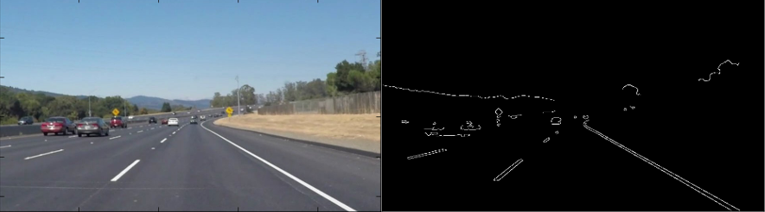
\includegraphics[width = 0.8\linewidth]{images/cannyEdgesExample.png}
  \caption{Beispiel: Fahrbahnbild und Canny-Edges-Filter}
  \label{fig:cannyExample}
\end{minipage}{
\vspace{0.8cm}
  
Der Canny-Edges-Filter wird im Kamera-Modul angewendet und über
\begin{lstlisting}
openCV.Canny("image-file", int lowerTreshold, int upperTreshold)
\end{lstlisting}
aufgerufen. Die Funktion liefert ein binäres Bild, das die Umrisse
  von Bildobjekten in weiß auf schwarzem Hintergrund darstellt
(siehe Abb.\ref{fig:cannyExample}).\\
Nach einem Rauschfilter, der im Hintergrund läuft, wird der Gradient
für jedes Pixel bestimmt. Liegt ein Gradient unterhalb des
\textit{untererThresholds},
wird ein Pixel schwarz im Zielbild, ist der Gradient oberhalb des
\textit{upperThresholds}, wird ein weißes Pixel ins Zielbild geschrieben. 
Gradientwerte im Zwischenbereich werden als schwarz geschrieben, es sei denn, 
sie sind mit Gradienten im Bild verbunden, die oberhalb des Thresholds liegen.\\
Die Einstellungen des Thresholds sind ein sensibler Bereich, da hier eine
Voretnscheidung getroffen wird, welche Bildinformationen erhalten bleiben bzw.
verworfen werden. Idealerweise würden hier nur die Umrisse der Fahrbanlinien
ausgewählt werden.\\

\subsubsection{Hough-Transformation}

\begin{minipage}{\columnwidth}
  \makeatletter
  \def\@captype{figure}
  \makeatother
  \centering
  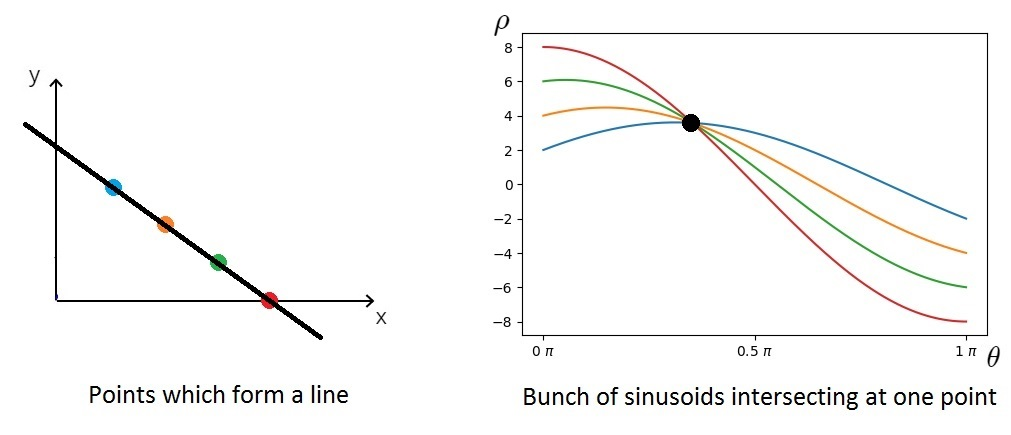
\includegraphics[width = 0.8\linewidth]{images/exampleHough.jpg}
  \caption{Beispiel: Darstellung einer Geraden kartesisch und im Hough-Raum}
  \label{fig:cannyExample}
\end{minipage}
\vspace{0.8cm}

Die Houghtransformation wird mit opencv.HoughLines(image, rho, theta, threshold) aufgerufen und gibt einen
Vektor zurück mit allen im Bild erkannten Lininen, die jeweils mit dem
Wertepaar($\rho$, $\theta$) beschrieben werden.Für $\rho$ und $\theta$ wird durch den Wert
ein Toleranzwert beschrieben. "threshold" bezeichnet einen Wert, der
die Mindestanzahl von Punkten bestimmt, die vorliegen müssen, damit eine Grade
als beschrieben gilt.\\
Die Funktion wird zweimal angewendet: zum Einen beim Start zur Initialisierung,
daß im gegeben Kamerabild die Fahrbahnlinien erkannt werden. Hierbei wird mit
einem größeren Toleranzbereich gearbeitet, um eine Erkennung sicherzustellen.
Zum anderen wird für jedes Bild des Kamerastreams die Linienerkennung gemacht,
und mit einem strengeren Toleranzbereich mit den aus dem Vorbild erkannten
Linienpaar verglichen. Dadurch soll verhindert werden, dass weitere erkannte
Linien, die nicht Teil der Fahrbahn sind, fehlerhaft in die erkannten Linien mit
einbezogen werden.\\
Die so noch erkannten Linien werden anhand von rho nd theta  entweder der linken 
oder der rechten Fahrbahnlinie zugeordnet, und für beide Seite eine Linie
gemittelt und als neue Orientierungslinen zur Richtungsbestimmung genutzt.\\
